

%----------------------------------------------------------------------------------------
%	PACKAGES AND OTHER DOCUMENT CONFIGURATIONS
%----------------------------------------------------------------------------------------

\documentclass[12pt]{article}

\usepackage{polski}
\usepackage[polish]{babel}
\usepackage[utf8]{inputenc}
\usepackage{datetime}
\usepackage{graphicx}
\usepackage{tikz}
\usepackage{amsmath}
\usepackage{epstopdf}
\usepackage{multirow}
\usepackage{tabularx}
%\usepackage[colorlinks=true]{hyperref}
%\usepackage[all]{hypcap}
%\usepackage{showframe} 
\usepackage{geometry}
 \geometry{
 a4paper, 
 left=20mm,
 right=20mm,
 top=20mm,
 bottom=20mm,
 }
 
%----------------------------------------------------------------------------------------
 
%----------------------------------------------------------------------------------------
% DATES
%----------------------------------------------------------------------------------------

\renewcommand{\dateseparator}{.}
\newdate{exercise_date}{25}{03}{2014}

%----------------------------------------------------------------------------------------

%----------------------------------------------------------------------------------------
% TIKZ PACKAGES
%----------------------------------------------------------------------------------------

\usetikzlibrary{arrows}

%----------------------------------------------------------------------------------------

\begin{document}
 
\begin{titlepage}

\newcommand{\HRule}{\rule{\linewidth}{0.5mm}}
% Defines a new command for the horizontal lines, change thickness here

\center
% Center everything on the page
 
%----------------------------------------------------------------------------------------
%	LOGO SECTION
%----------------------------------------------------------------------------------------

\includegraphics[width=6cm]{../res/img/logo.png}\\[1cm]
% Include a department/university logo - this will require the graphicx package
 
%----------------------------------------------------------------------------------------
 
%----------------------------------------------------------------------------------------
%	HEADING SECTIONS
%----------------------------------------------------------------------------------------

\textsc{\LARGE Akademia Górniczo-Hutnicza \\[0.2cm]
im. Stanisława Staszica w Krakowie}\\[1.5cm]
% Name of your university/college

\textrm{\Large Wydział Elektrotechniki Automatyki Informatyki i Inżynierii
Biomedycznej}\\[1cm]

\textsc{\Large Laboratorium Aparatury Automatyzacji}\\[0.5cm]
% Major heading such as course name

%----------------------------------------------------------------------------------------
%	TITLE SECTION
%----------------------------------------------------------------------------------------

\HRule \\[0.4cm]
{ \huge \bfseries Prosty regulator mikroprocesorowy 
}\\%[0.4cm]
% Title of your document
\HRule \\[1.5cm]

%----------------------------------------------------------------------------------------
%	REPORT TABLE
%----------------------------------------------------------------------------------------

\begin{table}[h]
\centering
\begin{tabularx}{\linewidth}{|c|l|X|}
\hline
% \multicolumn{3}{|c|}{
% \begin{tabular}{cc}
% \begin{tabular}{c}
% \includegraphics[height=2.2cm]{../res/img/logo.jpg}\\
% \end{tabular}
% &
% \begin{tabular}{c}
% \Large{Akademia Górniczo-Hutnicza im. Stanisława Staszica}\\[5pt]
% \large{\textsc{Katedra Automatyki}}\\[5pt]
% \textsc{Laboratorium Aparatury Automatyzacji}
% \end{tabular}
% \end{tabular}
% }\\
% \hline
% \multicolumn{3}{|c|}{}\\[-5pt]
% \multicolumn{3}{|c|}{\textbf{\huge{Ćwiczenie 6}}}\\[10pt]
% \multicolumn{3}{|c|}{\Large{Bezpośrednie sterowanie cyfrowe}}\\[8pt]
% \hline
\multicolumn{2}{|c|}{Wydział EAIiIB, kierunek AiR, rok II}
& Grupa 6, wtorek 11:00-12:30\\
\hline
Lp. & Imię i nazwisko & Zaliczenie\\
\hline
1 & \textbf{Konrad Adasiewicz} & \\
\hline
2 & \textbf{Michał Maciejewski} & \\
\hline
3 & \textbf{Bartosz Szmit} & \\
\hline
\multicolumn{2}{|c|}{Data wykonania ćwiczenia:
\ddmmyyyydate\displaydate{exercise_date}r.} & Data oddania sprawozdania:
\ddmmyyyydate\displaydate{create_date}r.
\\
\hline
\end{tabularx}
\end{table}

%----------------------------------------------------------------------------------------

\vfill % Fill the rest of the page with whitespace

\end{titlepage} 

\section{Wstęp teoretyczny} 

Celem ćwiczenia jest zapoznanie się z odpowiedziami skokowymi i impulsowymi
podstawowych obiektów dynamicznych. Obiekty dynamiczne automatyki opisywane są
transmitancją operatorową zdefiniowaną jako stosunek transformaty Laplace'a
sygnału wyjściowego z obiektu do transformaty Laplace'a sygnału wymuszającego,
przy założeniu zerowych warunków początkowych owych sygnałów w dziedzinie czasu:

\begin{equation*}
	G(s)=\frac{Y(s)}{U(s)}
\end{equation*}

Przy tak zdefiniowanej zależności wyznaczanie odpowiedzi operatorowych układów
nią opisanych jest bardzo proste i sprowadza się do obliczenia iloczynu
transformaty wymuszenia i transmitancji bloku.

Transformaty interesujących nas charakterystycznych wymuszeń to:

\begin{equation*}
	\mathcal{L}\{\delta(t)\}(s)=1
\end{equation*}

\begin{equation*}
	\mathcal{L}\{1(t)\}(s)=\frac{1}{s}
\end{equation*}

Zatem szukane odpowiedzi układów w dziedzinie czasu są dane zależnościami:

\begin{equation}
	y_{\delta}(t)=\mathcal{L}^{-1}\left\{G(s)\right\}
	\label{equ:tranimp}
\end{equation}

\begin{equation}
	y_1(t)=\mathcal{L}^{-1}\left\{\frac{1}{s}\cdot G(s)\right\}
	\label{equ:transtep}
\end{equation}

Gdzie $G(s)$ jest transmitancją badanego bloku.

Do uproszczenia analitycznego wyznaczenia odpowiedzi skokowej obiektu przydatna
jest zależność:

\begin{equation}
	y_1(t)=\int_0^t y_{\delta}(\tau)\mbox{d}\tau
\end{equation}

\newpage

\section{Odpowiedzi typowych układów dynamicznych w dziedzinie czasu}

We wszystkich transmitancjach wzmocnienie $k=1$. Odpowiedzi zostały wyznaczone
przy pomocy funkcji \textit{step} oraz \textit{impulse} dostępnych w pakiecie
matematycznym \textsc{Matlab}.

\subsection{Obiekt inercyjny I rzędu}

Transformata odpowiedzi impulsowej obiektu zgodnie ze wzorem \eqref{equ:tranimp}
wynosi:

\begin{equation*}
	Y_{\delta}(s)=\frac{1}{Ts+1}=\frac{1}{T}\cdot \frac{1}{s+\frac{1}{T}}
\end{equation*}

Transformata odwrotna:

\begin{equation*}
	y_{\delta}(t)=\mathcal{L}^{-1}\left\{\frac{1}{Ts+1}\right\}=
	\frac{1}{T}\cdot e^{-\frac{t}{T}}
\end{equation*}

\begin{figure}[!htb]
	\begin{center}
		\includegraphics[width=14cm]{../res/img/imp1.eps}
	\end{center}
	\caption{Odpowiedzi impulsowe obiektu inercyjnego I rzędu}
\end{figure}

\newpage

Transformata odpowiedzi skokowej obiektu zgodnie ze wzorem \eqref{equ:transtep}
wynosi:

\begin{equation*}
	Y_{1}(s)=\frac{1}{s}\cdot \frac{1}{Ts+1}=\frac{1}{s}\cdot \frac{1}{T}\cdot
	\frac{1}{s+\frac{1}{T}}
\end{equation*}

Transformata odwrotna:

\begin{equation*}
	y_{1}(t)=\mathcal{L}^{-1}\left\{\frac{1}{s}\cdot \frac{1}{Ts+1}\right\} =
	1-e^{-\frac{t}{T}}
\end{equation*}

\begin{figure}[!htb]
	\begin{center}
		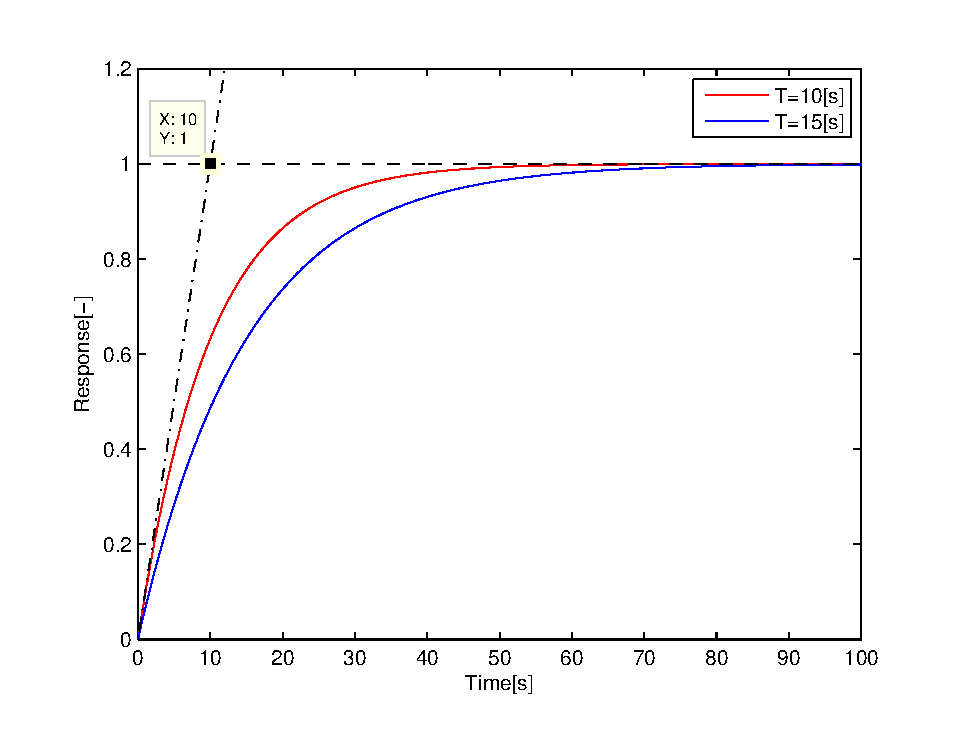
\includegraphics[width=14cm]{../res/img/step1.eps}
	\end{center}
	\caption{Odpowiedzi skokowe obiektu inercyjnego I rzędu}
\end{figure}

Na wykresie odpowiedzi impulsowej został zaznaczony charakterystyczny punkt,
dzięki któremu można odczytać czas inercji obiektu z uwagi na to iż
prawostronna granica odpowiedzi w zerze jest równa $\frac{1}{T}$. Dodatkowo na
wykresie odpowiedzi skokowej została zaprezentowana graficzna metoda wyznaczenia
czasu inercji obiektu. W analogiczny sposób można również wyznaczyć czas
opóźnienia z charakterystyki impulsowej. Szukany czas jest czasem po którym
wrysowana styczna osiągnie wartość do której obiekt dąży w stanie ustalonym.

\newpage

\subsection{Obiekt inercyjny II rzędu}

Transformata odpowiedzi impulsowej obiektu zgodnie ze wzorem \eqref{equ:tranimp}
wynosi:

\begin{equation*}
	Y_{\delta}(s)=\frac{1}{(T_1s+1)(T_2s+1)} =
		\frac{1}{T_1-T_2}\cdot \frac{1}{s+\frac{1}{T_1}}+
		\frac{1}{T_2-T_1}\cdot \frac{1}{s+\frac{1}{T_2}}
\end{equation*}

Transformata odwrotna:

\begin{equation*}
	y_{\delta}(t)=\mathcal{L}^{-1}\left\{\frac{1}{(T_1s+1)(T_2s+1)}\right\} =
		\frac{1}{T_1-T_2}\cdot e^{-\frac{t}{T_1}}+
		\frac{1}{T_2-T_1}\cdot e^{-\frac{t}{T_2}}
\end{equation*}

\begin{figure}[!htb]
	\begin{center}
		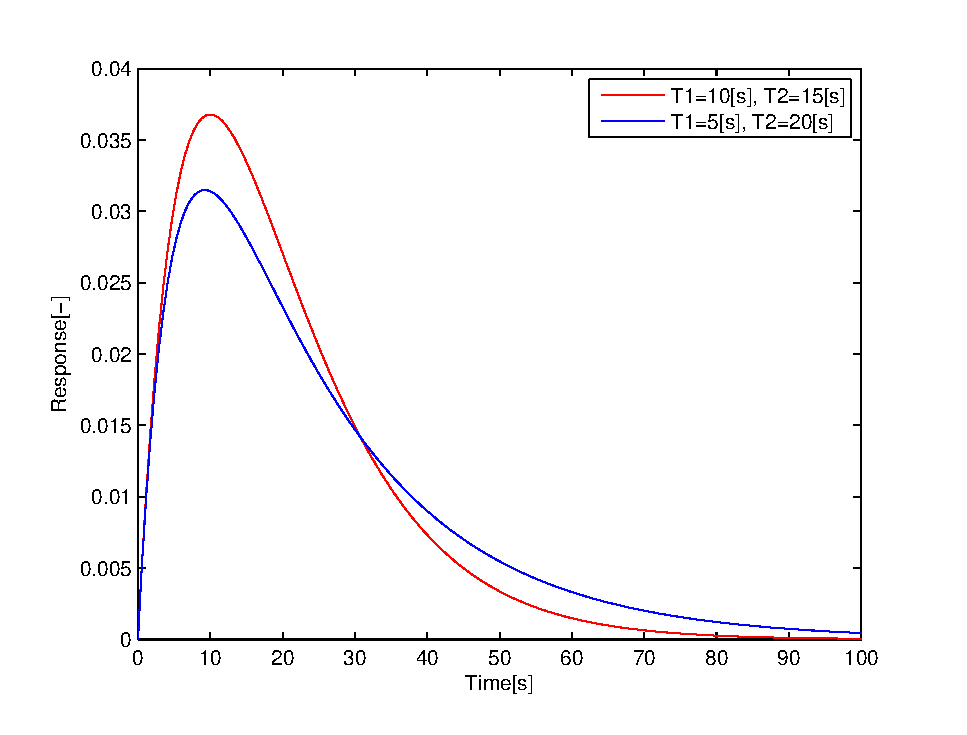
\includegraphics[width=14cm]{../res/img/imp2.eps}
	\end{center}
	\caption{Odpowiedzi impulsowe obiektu inercyjnego II rzędu}
\end{figure}

\newpage

Transformata odpowiedzi skokowej obiektu zgodnie ze wzorem \eqref{equ:transtep}
wynosi:

\begin{equation*}
	Y_{1}(s)=\frac{1}{s(T_1s+1)(T_2s+1)}=
	\frac{1}{s}-
	\frac{T_1}{T_1-T_2}\cdot \frac{1}{s+\frac{1}{T_1}}-
	\frac{T_2}{T_2-T_1}\cdot \frac{1}{s+\frac{1}{T_2}}
\end{equation*}

Transformata odwrotna:

\begin{equation*}
	y_{1}(t)=\mathcal{L}^{-1}\left\{\frac{1}{s(T_1s+1)(T_2s+1)}\right\}=
	1-
	\frac{T_1}{T_1-T_2}\cdot e^{-\frac{t}{T_1}}-
	\frac{T_2}{T_2-T_1}\cdot e^{-\frac{t}{T_2}}
\end{equation*}

\begin{figure}[!htb]
	\begin{center}
		\includegraphics[width=14cm]{../res/img/step2.eps}
	\end{center}
	\caption{Odpowiedzi skokowe obiektu inercyjnego II rzędu}
\end{figure}

Obiekt inercyjny rzędu II jest obiektem trudnym do analizy, ponieważ na
podstawie jego charakterystyk skokowej i impulsowej nie jesteśmy w stanie w
prosty sposób wyznaczyć żadnych jego parametrów. Dlatego w praktycznych
zastosowaniach obiekty inercyjne wyższych rzędów opisuje się przy pomocy
uproszczonego modelu obiektu inercyjnego I rzędu z opóźnieniem.

\newpage

\subsection{Obiekt oscylacyjny II rzędu}

Transformata odpowiedzi impulsowej obiektu zgodnie ze wzorem \eqref{equ:tranimp}
wynosi:

\begin{equation*}
	Y_{\delta}(s)=\frac{1}{T_0^2s^2+2\xi T_0s+1}
\end{equation*}

Transformata odwrotna:

\begin{equation*}
	y_{\delta}(t)=\mathcal{L}^{-1}\left\{\frac{1}{T_0^2s^2+2\xi T_0s+1}\right\} =
	\frac{1}{T_0}\cdot \frac{1}{\sqrt{1-\xi^2}} \cdot e^{-\frac{\xi}{T_0}t} 
	\cdot \sin\left(\frac{\sqrt{1-\xi^2}}{T_0}t\right)
\end{equation*}

\begin{figure}[!htb]
	\begin{center}
		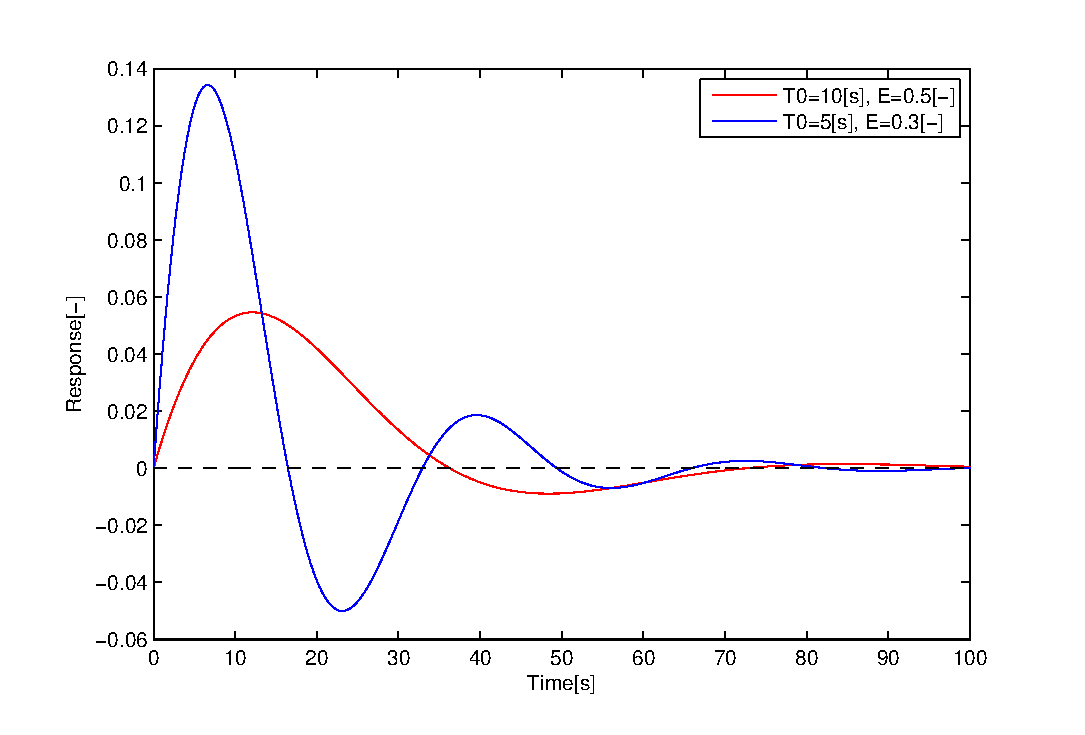
\includegraphics[width=14cm]{../res/img/imp3.eps}
	\end{center}
	\caption{Odpowiedzi impulsowe obiektu oscylacyjnego II rzędu}
\end{figure}

\newpage

Transformata odpowiedzi skokowej obiektu zgodnie ze wzorem \eqref{equ:transtep}
wynosi:

\begin{equation*}
	Y_{1}(s)=\frac{1}{s(T_0^2s^2+2\xi T_0s+1)}
\end{equation*}

Transformata odwrotna:

\begin{equation*}
	y_{1}(t)=\mathcal{L}^{-1}\left\{\frac{1}{s(T_0^2s^2+2\xi T_0s+1)}\right\}
\end{equation*}

Nie jesteśmy w stanie przytoczyć analitycznej zależności na ogólną odpowiedź
skokową obiektu oscylacyjnego z uwagi na jej skomplikowaną postać.

\begin{figure}[!htb]
	\begin{center}
		\includegraphics[width=14cm]{../res/img/step3.eps}
	\end{center}
	\caption{Odpowiedzi skokowe obiektu oscylacyjnego II rzędu}
\end{figure}

Obiekt oscylacyjny rzędu II charakteryzują dwa parametry, czas charakterystyczny
$T_0$ oraz tłumienie $\xi$. Obydwa z nich można wyznaczyć znając zarówno
odpowiedź impulsową jak i skokową. W tym celu należy wyznaczyć okres oscylacji
odpowiedzi $T_r$ oraz logarytmiczny dekrement tłumienia $\Lambda$ zdefiniowany
jako iloraz amplitud dwóch kolejnych drgań odpowiedzi tego samego znaku:

\begin{equation*}
	\Lambda = \ln{\frac{y_{n+1}}{y_{n}}}
\end{equation*}

Wtedy:

\begin{equation*}
	\xi = \left|\frac{\Lambda}{\sqrt{4\pi^2+\Lambda^2}}\right| \hspace{1cm}
	T_0 = \frac{T_r\sqrt{1-\xi^2}}{2\pi}
\end{equation*}

\newpage

\subsection{Obiekt całkujący z inercją I rzędu}

Transformata odpowiedzi impulsowej obiektu zgodnie ze wzorem \eqref{equ:tranimp}
wynosi:

\begin{equation*}
	Y_{\delta}(s)=\frac{1}{T_is(Ts+1)}=\frac{1}{T_i}\left(\frac{1}{s} -
	\frac{T}{Ts+1}\right)
\end{equation*}

Transformata odwrotna:

\begin{equation*}
	y_{\delta}(t)=\mathcal{L}^{-1}\left\{\frac{1}{T_is(Ts+1)}\right\} =
	\frac{1}{T_i}\left(1-e^{-\frac{t}{T}}\right)
\end{equation*}

\begin{figure}[!htb]
	\begin{center}
		\includegraphics[width=14cm]{../res/img/imp4.eps}
	\end{center}
	\caption{Odpowiedzi impulsowe obiektu całkującego z inercją I rzędu}
\end{figure}

\newpage

Transformata odpowiedzi skokowej obiektu zgodnie ze wzorem \eqref{equ:transtep}
wynosi:

\begin{equation*}
	Y_{1}(s)=\frac{1}{T_is^2(Ts+1)}=\frac{1}{T_i}\left(\frac{1}{s^2} -
	\frac{T}{s} +	\frac{T^2}{Ts+1}\right)
\end{equation*}

Transformata odwrotna:

\begin{equation*}
	y_{1}(t)=\mathcal{L}^{-1}\left\{\frac{1}{T_is^2(Ts+1)}\right\} =
	\frac{1}{T_i}\left(t - T + Te^{-\frac{t}{T}}\right)
\end{equation*}

\begin{figure}[!htb]
	\begin{center}
		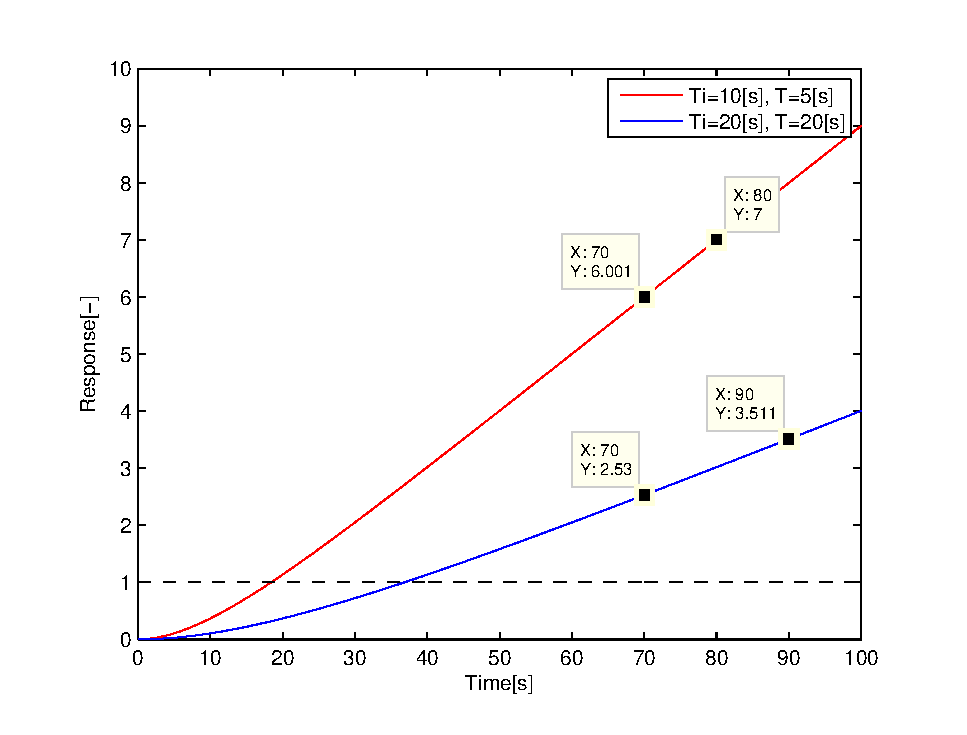
\includegraphics[width=14cm]{../res/img/step4.eps}
	\end{center}
	\caption{Odpowiedzi skokowe obiektu całkującego z inercją I rzędu}
\end{figure}

W przypadku obiektu całkującego z inercją, na podstawie charakterystyki
impulsowej jesteśmy w stanie oba parametry obiektu, tj. czas całkowania $T_i$,
który obliczamy, na podstawie wartości odpowiedzi w stanie ustalonym(powinna
ona wynosić $\frac{1}{T_i}$) oraz stałą czasową inercji $T$, którą wyznaczamy
identycznie jak w przypadku obiektu inercyjnego rzędu I. Natomiast z uwagi na
obecność akcji całkującej w obiekcie nie jesteśmy w stanie wyznaczyć stałej
czasowej tylko na podstawie przebiegu odpowiedzi skokowej układu. Możemy
natomiast po zaniknięciu inercji wyznaczyć czas całkowania na podstawie
szybkości narastania odpowiedzi(powinna narastać jak $\frac{1}{T_i}t$).

\newpage

\subsection{Obiekt różniczkujący rzeczywisty}

Transformata odpowiedzi impulsowej obiektu zgodnie ze wzorem \eqref{equ:tranimp}
wynosi:

\begin{equation*}
	Y_{\delta}(s)=\frac{T_ds}{Ts+1}=
	\frac{T_d}{T}\left(1 - \frac{1}{Ts+1}\right)
\end{equation*}

Transformata odwrotna:

\begin{equation*}
	y_{\delta}(t)=\mathcal{L}^{-1}\left\{\frac{T_ds}{Ts+1}\right\} =
	\frac{T_d}{T}\left(\delta(t)-\frac{1}{T}e^{-\frac{t}{T}}\right)
\end{equation*}

\begin{figure}[!htb]
	\begin{center}
		\includegraphics[width=14cm]{../res/img/imp5.eps}
	\end{center}
	\caption{Odpowiedzi impulsowe obiektu różniczkującego rzeczywistego}
\end{figure}

\newpage

Transformata odpowiedzi skokowej obiektu zgodnie ze wzorem \eqref{equ:transtep}
wynosi:

\begin{equation*}
	Y_{1}(s)=\frac{T_d}{Ts+1}=\frac{T_d}{T}\cdot \frac{1}{s+\frac{1}{T}}
\end{equation*}

Transformata odwrotna:

\begin{equation*}
	y_{1}(t)=\mathcal{L}^{-1}\left\{\frac{T_d}{Ts+1}\right\} =
	\frac{T_d}{T}e^{-\frac{t}{T}}
\end{equation*}

\begin{figure}[!htb]
	\begin{center}
		\includegraphics[width=14cm]{../res/img/step5.eps}
	\end{center}
	\caption{Odpowiedzi skokowe obiektu różniczkującego rzeczywistego}
\end{figure}

Ponieważ w rzeczywistym świecie nie występuje obiekt różniczkujący idealny,
rozpatruje się połączenie obiektu różniczkującego z inercyjnym I rzędu. Czas
inercji $T$ tego obiektu odczytujemy analogicznie jak w przypadku samego członu
inercyjnego, natomiast czas wyprzedzenia obliczamy znając wartość $T$ oraz
granicę prawostronną wartości odpowiedzi w czasie $t=0^{+}$. Powinna ona wynosić
odpowiednio $-\frac{T_d}{T^2}$ dla odpowiedzi impulsowej oraz $\frac{T_d}{T}$
dla charakterystyki skokowej.

\newpage

\subsection{Obiekt inercyjny I rzędu z opóźnieniem}

Transformata odpowiedzi impulsowej obiektu zgodnie ze wzorem \eqref{equ:tranimp}
wynosi:

\begin{equation*}
	Y_{\delta}(s)=\frac{e^{-s\tau}}{Ts+1}
\end{equation*}

Transformata odwrotna:

\begin{equation*}
	y_{\delta}(t)=\mathcal{L}^{-1}\left\{\frac{e^{-s\tau}}{Ts+1}\right\} =
	1(t-\tau)\cdot \frac{1}{T}\cdot e^{-\frac{t-\tau}{T}}
\end{equation*}

\begin{figure}[!htb]
	\begin{center}
		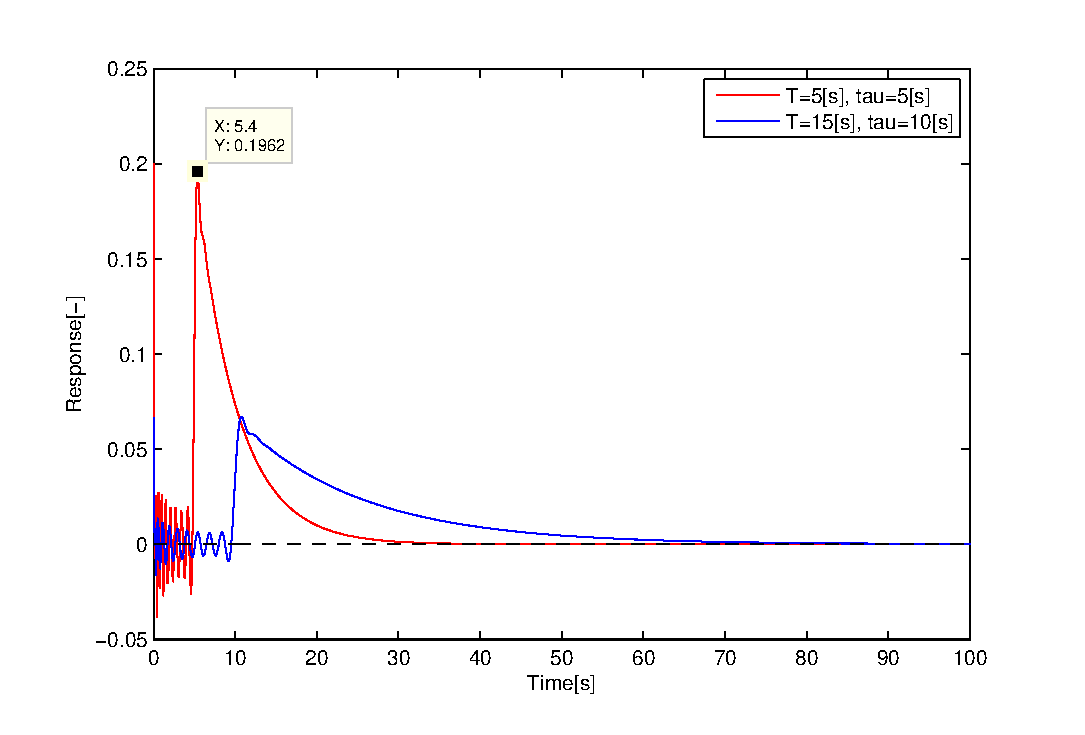
\includegraphics[width=14cm]{../res/img/imp6.eps}
	\end{center}
	\caption{Odpowiedzi impulsowe obiektu inercyjnego I rzędu z opóźnieniem}
\end{figure}

\newpage

Transformata odpowiedzi skokowej obiektu zgodnie ze wzorem \eqref{equ:transtep}
wynosi:

\begin{equation*}
	Y_{1}(s)=\frac{e^{-s\tau}}{s(Ts+1)}
\end{equation*}

Transformata odwrotna:

\begin{equation*}
	y_{1}(t)=\mathcal{L}^{-1}\left\{\frac{e^{-s\tau}}{s(Ts+1)}\right\} =
	1(t-\tau)\cdot \left(1-e^{-\frac{t-\tau}{T}}\right)
\end{equation*}

\begin{figure}[!htb]
	\begin{center}
		\includegraphics[width=14cm]{../res/img/step6.eps}
	\end{center}
	\caption{Odpowiedzi skokowe obiektu inercyjnego I rzędu z opóźnieniem}
\end{figure}

Występujące w czasie martwym oscylacje odpowiedzi występują ze względu na fakt
aproksymowania członu opóźniającego transmitancją Pade'go z uwagi na to, iż nie
może ona zostać zapisana w postaci skończonego ułamka wymiernego transmitancji.
Czas martwy $\tau$ to czas w którym odpowiedź nie reaguje jeszcze na wymuszenie,
poza tym obiekt analizujemy tak jak zwykły obiekt inercyjny.

\newpage

\section{Wnioski i spostrzeżenia}

Na podstawie analizowanych odpowiedzi skokowych i~impulsowych można zauważyć, że
nie z~każdej odpowiedzi umieszczonej na wykresie można odczytać parametry
obiektu. Dla przykładu, obiekt II rzędu posiada dwie stałe czasowe $T_1$ oraz
$T_2$, których identyfikacja na wykresie jest bardzo trudna, a~czasem wręcz
niemożliwa.

W sprawozdaniu zostały opisane metody identyfikacji parametrów obiektów, gdyż
znajomość metodyki ich odczytywania z odpowiedzi standardowych jest naszym
zdaniem wystarczającym wyznacznikiem znajomości ich wpływu na przebieg
odpowiedzi.

\end{document}